\begin{slikaDesno}{fig/LC_izbijanje.pdf}
    \textbf{{\color{red}*}\ID.} 
    У колу са слике познати су 
    $L$, 
    $C$ и коефицијент магнетске спреге $k \ll 1$.
    У почетном тренутку су познати 
    $i_2(0) = v_1(0) = v_2(0) = 0$ и 
    $i_1(0) = I_0$. Поставити (а)
    систем 
    интегро-диференцијалних једначина кола 
    по струјама $i_1$ и $i_2$. Помоћу 
    Лапласове
    трансформације (б) одредити струју $i_1(t)$.
    Скицирати (в) временски дијаграм 
    добијеног одзива
    $i_1(t)$ за $t > 0$.
\end{slikaDesno} \\

\textsc{\underline{Решење}}:
Напоне $v_1$ и $v_2$ са једне стране повезују струјно-напонске карактеристике
спрегнутих калемова дата је системом једначина 
\begin{eqnarray}
    v_1 = L_1 \dfrac{\de i_1}{\de t} + L_{12} \dfrac{\de i_2}{\de t} \\
    v_2 = L_{21} \dfrac{\de i_1}{\de t} + L_{2} \dfrac{\de i_2}{\de t},
\end{eqnarray}
При чему су, по услову задатка, $L_1 = L_2 = L$ и $L_{12} = L_{21} = kL$. Са друге стране, 
напон и струја су повезани према карактеристици кондензатора\footnote{
Полазећи од израза за струја што се може записати у интегралној форми као 
$\DS v_{\rm 1} = - \dfrac{1}{C} \int_{0}^{t} i_1 \de \uptau$, односно
$\DS v_{\rm 2} = - \dfrac{1}{C} \int_{0}^{t} i_2 \de \uptau$.
Заменом у израз за струју кондензатора $i_{\rm C} = C \dfrac{\de v_C}{\de t}$, интеграљењем
обе стране се добија коришћена напонско-струјна карактеристика.
} при неусклађеним референтним 
смеровима резултата, у систем једначина спрегнутих калемова и даљим сређивањем добија се 
\begin{eqnarray}
    - \dfrac{1}{C} \int_{0}^{t} i_1 \de \uptau = L \dfrac{\de i_1}{\de t} + kL \dfrac{\de i_2}{\de t}; 
    & \Rightarrow & 
    \dfrac{\de i_1}{\de t} + k \dfrac{\de i_2}{\de t} + \upomega_0^2 \int_0^t i_1 \, \de \uptau = 0
    \\
    - \dfrac{1}{C} \int_{0}^{t} i_2 \de \uptau = kL \dfrac{\de i_1}{\de t} + L \dfrac{\de i_2}{\de t}
    & \Rightarrow &
    k \dfrac{\de i_1}{\de t} + \dfrac{\de i_2}{\de t} + \upomega_0^2 \int_0^t i_2 \, \de \uptau = 0,
\end{eqnarray}
где је $\upomega_0 = \dfrac{1}{\sqrt{LC}}$. Добијени систем интегро-диференцијалних једначина 
описује понашање посматраног система \\

(б) Добијени систем једначина преводи се у фреквенцијски домен применом правила диференцирања 
уз почетни услов\ и правила интеграљења\footnote{Правило диференцирања $\mathcal{L} \left\{ \dfrac{\de x(t)}{\de t} \right\}
= s X(s) - x(0^+)$; Правило интеграљења 
$\DS \mathcal{L} \left\{ \int_{0^-}^{t} f(\uptau) \, \de \uptau \right\} = \dfrac{1}{s} F(s)$. }. 
Нека су $I_1 = I_1(s)$ и $I_2 = I_2(s)$, онда је
\begin{eqnarray}
    sI_1 - I_0 + ksI_2 + \dfrac{\upomega_0^2}{s} I_1 = 0
    & \Rightarrow & 
    (s^2 + \upomega_0^2) I_1 + ks^2 I_2 = I_0 s \\
    ksI_1 - kI_0 + sI_2 + \dfrac{\upomega_0^2}{s} I_2 = 0
    & \Rightarrow & 
    ks^2 I_1 + (s^2 + \upomega_0^2) I_2 = k I_0 s
\end{eqnarray}
Решавањем добијеног система једначина по непознатим струјама добијају се резултати: 
\begin{eqnarray}
    I_1 &=& \frac{I_{0} s \bigl(s^{2} \left(k^{2} - 1\right) - \upomega_{0}^{2} \bigr)}{\bigl(s^{2} \left(k - 1\right) - \upomega_{0}^{2} \bigr) \left(s^{2} \left(k + 1\right) + \upomega_{0}^{2}\right)} \\[2mm]
    I_2 &=& - \frac{I_{0} \upomega_{0}^{2} k s}{\bigl(s^{2} \left(k - 1\right) - \upomega_{0}^{2} \bigr) \left(s^{2} \left(k + 1\right) + \upomega_{0}^{2}\right)}
    \label{eq:\ID_i2s}
\end{eqnarray}
Добијени резултати за струје се растављају на парцијалне разломке у односу на променљиву 
$s^2$ (практично се уводи смена). Прво се раставља израз за струју $I_1$ на парцијалне разломке
као
\begin{eqnarray}
    &I_1 = \dfrac{A}{s^2(1 - k) + \upomega_0^2} + \dfrac{B}{s^2(1+k) + \upomega_0^2} \\ 
    &
    \begin{cases}
    A = 
    \left.
    \frac{I_{0} s \bigl(s^{2} \left(k^{2} - 1\right) - \upomega_{0}^{2} \bigr)}
    { \cancel{\bigl(s^{2} \left(k - 1\right) - \upomega_{0}^{2} \bigr)} \left(s^{2} \left(k + 1\right) + \upomega_{0}^{2}\right)}
    \right\rvert_{s^2 = \frac{\upomega_0^2}{k-1}}
    = -I_0 s \dfrac{1-k}{2} 
        \\    
    B = \left.
        \frac{I_{0} s \bigl(s^{2} \left(k^{2} - 1\right) - \upomega_{0}^{2} \bigr)}
        { \bigl(s^{2} \left(k - 1\right) - \upomega_{0}^{2} \bigr) \cancel{\left(s^{2} \left(k + 1\right) + \upomega_{0}^{2}\right)}}
    \right\rvert_{s^2 = -\frac{\upomega_0^2}{1 + k}}
    = I_0 s \dfrac{1+k}{2}
    \end{cases}
\end{eqnarray}
Коначно се добија поједностављен облик струје $I_1 = 
\dfrac{I_0}{2} \left(  
    \dfrac{s}{s^2 + \dfrac{\upomega_0^2}{k+1} }
    +
    \dfrac{s}{s^2 + \dfrac{\upomega_0^2}{1-k}}
\right)$,
а облик у временском домену се одређује непосредном идентификацијом табличних 
транформација\footnote{Релевантна таблична трансформација је 
$\mathcal{L} \{ \cos(\upomega_0 t) \} = \dfrac{s}{s^2 + \upomega_0^2} $}
$i_1(t) = \dfrac{I_0}{2} 
\Biggl(
    \cos \left( \dfrac{\upomega_0}{\sqrt{1+k}}t\right) + \cos\left(\dfrac{\upomega_0}{\sqrt{1-k}}t\right) 
\Biggr)$. 

Друга струја се налази на сличан аналоган начина растављањем израза 
\eqref{eq:\ID_i2s} на парцијалне разломке: 
\begin{eqnarray}
    &I_2 = \dfrac{A}{s^2(1 - k) + \upomega_0^2} + \dfrac{B}{s^2(1+k) + \upomega_0^2} \\ 
    &
    \begin{cases}
    A = 
    \left.
    \frac{I_{0} \upomega_{0}^{2} k s}
    { \cancel{\bigl(s^{2} \left(k - 1\right) - \upomega_{0}^{2} \bigr)} \left(s^{2} \left(k + 1\right) + \upomega_{0}^{2}\right)}
    \right\rvert_{s^2 = \frac{\upomega_0^2}{k-1}}
    = I_0 s \dfrac{1-k}{2} 
        \\    
    B = \left.
        \frac{I_{0} \upomega_{0}^{2} k s}
        { \bigl(s^{2} \left(k - 1\right) - \upomega_{0}^{2} \bigr) \cancel{\left(s^{2} \left(k + 1\right) + \upomega_{0}^{2}\right)}}
    \right\rvert_{s^2 = -\frac{\upomega_0^2}{1 + k}}
    = I_0 s \dfrac{1+k}{2}
    \end{cases}
\end{eqnarray}
   Одакле се има резултат 
    $I_2 = 
\dfrac{I_0}{2} \left(  
    \dfrac{s}{s^2 + \dfrac{\upomega_0^2}{k+1} }
    -
    \dfrac{s}{s^2 + \dfrac{\upomega_0^2}{1-k}}
\right)$. Примећујемо да се резултат за ову струју разликује само по знаку једног члана од 
комплексне струје $I_1$, самим тим, резултат у временском домену је 
$i_2(t) = \dfrac{I_0}{2} 
\Biggl(
    \cos \left( \dfrac{\upomega_0}{\sqrt{1+k}}t\right) - \cos\left(\dfrac{\upomega_0}{\sqrt{1-k}}t\right) 
\Biggr)$. 

\begin{figure}[t!]
    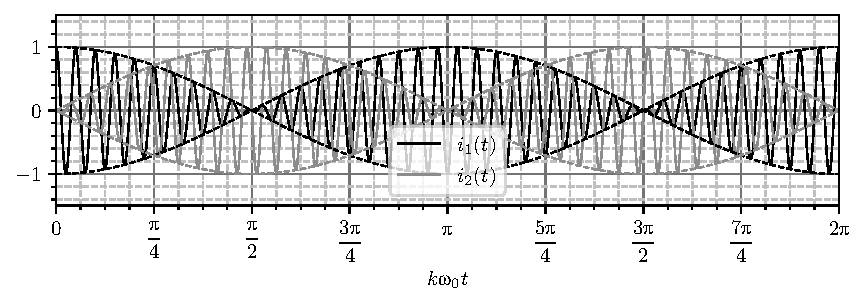
\includegraphics[scale=1]{fig/LC_plot.pdf}
    \caption{Илустрација резултата.}
    \label{fig:\ID.2}
\end{figure}

(в) Уколико се по претпоставци усвоји да је $k\ll1$ онда се може 
апроксимирати\footnote{Користи се апроксимација првим чланом Тејлоровог развоја
$(1 + x)^{\upalpha} \approx 1 + \upalpha x$, за $\upalpha = -\dfrac{1}{2}$.}
да је $\dfrac{1}{\sqrt{1 \pm k}} = 1 \mp \dfrac{1}{2}k$. Погоднији облик струја се може добити 
изражавањем збира, односно разлике косинуса преко производа\footnote{ Одговарајући тригонометријски идентитети јесу
$\cos x + \cos y = 2 \cos\left(\dfrac{x+y}{2}\right)\cos\left(\dfrac{x-y}{2}\right)$, 
и $\cos x - \cos y = - \sin\left(\dfrac{x+y}{2}\right)\sin\left(\dfrac{x-y}{2}\right)$}. има се приближни
резултат:
\begin{eqnarray}
    & i_1(t) \approx I_0 \cos(2\upomega_0 t) \cos( k\upomega_0 t ), \\
    & i_2(t) \approx -I_0 \sin(2\upomega_0 t) \sin( k\upomega_0 t ).
\end{eqnarray}
Добијени резултати приказани су на графику на слици \ref{fig:\ID.2}. На слици пуном линијом 
су приказани одговарајући сигнали. Испрекиданим линијама приказане су анвелопе тих сигнала, 
које илуструју процес „шетања“ енергије између једног и другог осцилаторног кола. 
Појава која је добијена дешава се у општем случају у систему спрегнутих осцилатора. 


